
\documentclass{article}[14pt]
\usepackage{multicol, enumerate, enumitem, hyperref, color, soul, setspace, parskip, fancyhdr, amssymb, amsthm, amsmath, bbm, latexsym, units, mathtools}
\everymath{\displaystyle}
\usepackage[headsep=0.5cm,headheight=0cm, left=1 in,right= 1 in,top= 1 in,bottom= 1 in]{geometry}
\pagestyle{fancy}
\lhead{}
\chead{Answer Key for Module\,7\,-\,Rational\,Functions Version A}
\rhead{}
\lfoot{Summer\,C\,2020}
\cfoot{}
\rfoot{}
\begin{document}
\textbf{This key should allow you to understand why you choose the option you did (beyond just getting a question right or wrong). \href{https://xronos.clas.ufl.edu/mac1105spring2020/courseDescriptionAndMisc/Exams/LearningFromResults}{More instructions on how to use this key can be found here}.}

\textbf{If you have a suggestion to make the keys better, \href{https://forms.gle/CZkbZmPbC9XALEE88}{please fill out the short survey here}.}

\textit{Note: This key is auto-generated and may contain issues and/or errors. The keys are reviewed after each exam to ensure grading is done accurately. If there are issues (like duplicate options), they are noted in the offline gradebook. The keys are a work-in-progress to give students as many resources to improve as possible.}

\rule{\textwidth}{0.4pt}

31. Solve the rational equation below. Then, choose the interval(s) that the solution(s) belongs to.
$$ \frac{-48}{-32x -32} + 1 = \frac{-48}{-32x -32} $$ 
The solution is $ \text{all solutions are invalid or lead to complex values in the equation.} $ 

\begin{enumerate}[label=\Alph*.] 
\item $ x \in [-0.8,2.8] $ 

 $x = 1.000$, which corresponds to not distributing the factor $-32x -32$ correctly when trying to eliminate the fraction. 
\item $ x_1 \in [-1.5, 0.6] \text{ and } x_2 \in [0,3] $ 

 $x = -1.000 \text{ and } x = 1.000$, which corresponds to getting the correct solution and believing there should be a second solution to the equation. 
\item $ x_1 \in [-1.5, 0.6] \text{ and } x_2 \in [-6,0] $ 

 $x = -1.000 \text{ and } x = -1.000$, which corresponds to getting the correct solution and believing there should be a second solution to the equation. 
\item $ \text{All solutions lead to invalid or complex values in the equation.} $ 

 *$x = -1.000$ leads to dividing by 0 in the original equation and thus is not a valid solution, which is the correct option. 
\item $ x \in [-1.0,0.0] $ 

 $x = -1.000$, which corresponds to not checking if this value leads to dividing by 0 in the original equation and thus is not a valid solution. 
\end{enumerate} 
 
General Comments: Distractors are different based on the number of solutions. Remember that after solving, we need to make sure our solution does not make the original equation divide by zero!

-----------------------------------------------

32. Solve the rational equation below. Then, choose the interval(s) that the solution(s) belongs to.
$$ \frac{-6x}{6x + 6} + \frac{-7x^{2}}{-36x^{2} -72 x -36} = \frac{-6}{-6x -6} $$ 
The solution is $ \text{There are two solutions: } x = -1.789 \text{ and } x = -0.694 $ 

\begin{enumerate}[label=\Alph*.] 
\item $ x_1 \in [-2.23, -1.62] \text{ and } x_2 \in [-0.82,-0.6] $ 

 * $x = -1.789 \text{ and } x = -0.694$, which is the correct option. 
\item $ \text{All solutions lead to invalid or complex values in the equation.} $ 

  
\item $ x \in [-0.96,-0.4] $ 

  
\item $ x_1 \in [-2.23, -1.62] \text{ and } x_2 \in [-1.06,-0.79] $ 

  
\item $ x \in [-1,-0.96] $ 

  
\end{enumerate} 
 
General Comments: Distractors are different based on the number of solutions. Remember that after solving, we need to make sure our solution does not make the original equation divide by zero!

-----------------------------------------------

33. Determine the domain of the function below.
$$ f(x) = \frac{4}{20x^{2} -4 x -24} $$ 
The solution is $ \text{All Real numbers except } x = -1.000 \text{ and } x = 1.200. $ 

\begin{enumerate}[label=\Alph*.] 
\item $ \text{All Real numbers.} $ 

 This corresponds to thinking the denominator has complex roots or that rational functions have a domain of all Real numbers. 
\item $ \text{All Real numbers except } x = a, \text{ where } a \in [-3, 0] $ 

 All Real numbers except $x = -1.000$, which corresponds to removing only 1 value from the denominator. 
\item $ \text{All Real numbers except } x = a \text{ and } x = b, \text{ where } a \in [-21, -15] \text{ and } b \in [29, 34] $ 

 All Real numbers except $x = -16.000$ and $x = 30.000$, which corresponds to not factoring the denominator correctly. 
\item $ \text{All Real numbers except } x = a, \text{ where } a \in [-21, -15] $ 

 All Real numbers except $x = -16.000$, which corresponds to removing a distractor value from the denominator. 
\item $ \text{All Real numbers except } x = a \text{ and } x = b, \text{ where } a \in [-3, 0] \text{ and } b \in [0, 2] $ 

 All Real numbers except $x = -1.000$ and $x = 1.200$, which is the correct option. 
\end{enumerate} 
 
General Comments: The new domain is the intersection of the previous domains.

-----------------------------------------------

34. Choose the graph of the equation below.
$$ f(x) = \frac{-1}{(x - 1)^2} - 3 $$ 

 
 The solution is  
 \begin{center} 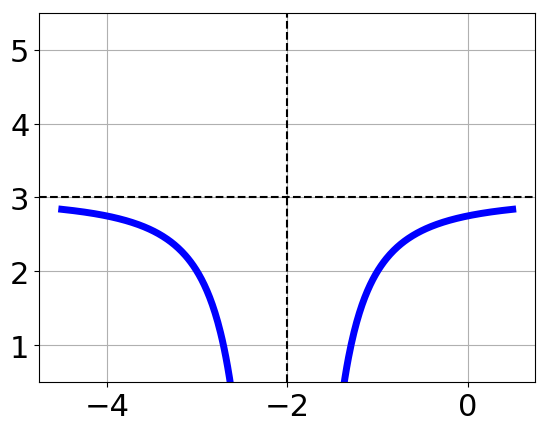
\includegraphics[width=0.3\textwidth]{../Figures/rationalEquationToGraphAB.png} \end{center}\begin{tabular}{|c|c|} 
\hline 
 & \tabularnewline 
 \textbf{A.} 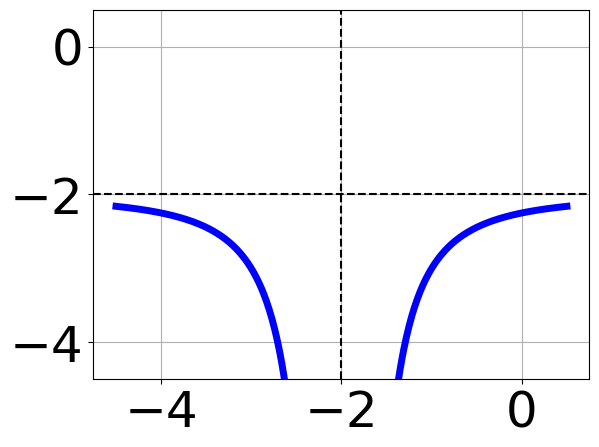
\includegraphics[width=0.3\textwidth]{../Figures/rationalEquationToGraphAA.png} & \textbf{B.} 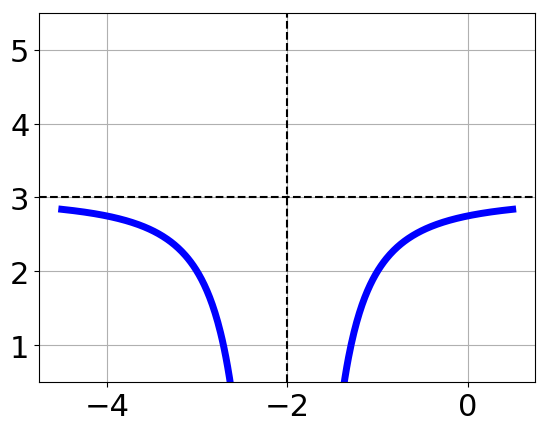
\includegraphics[width=0.3\textwidth]{../Figures/rationalEquationToGraphAB.png} \tabularnewline 
\hline 
 & \tabularnewline 
 \textbf{C.} 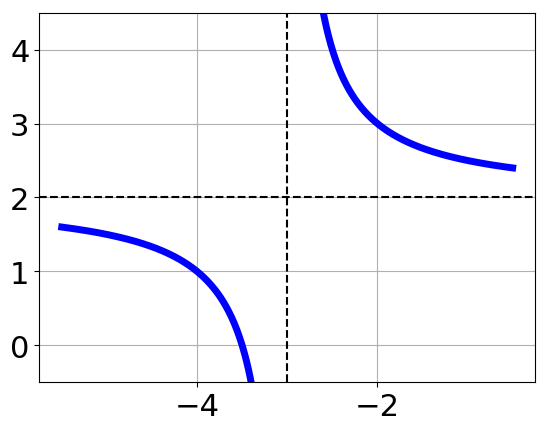
\includegraphics[width=0.3\textwidth]{../Figures/rationalEquationToGraphAC.png} & \textbf{D.} 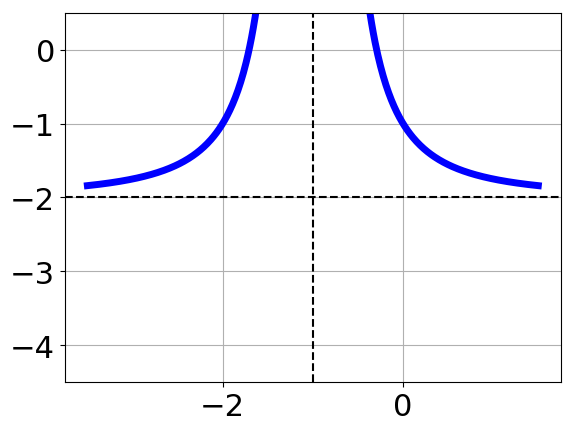
\includegraphics[width=0.3\textwidth]{../Figures/rationalEquationToGraphAD.png} \tabularnewline 
\hline 
 E. None of the figures above. & \tabularnewline 
\hline 
 \end{tabular} 
 
General Comments: Remember that the general form of a basic rational equation is $ f(x) = \frac{a}{(x-h)^n} + k$, where $a$ is the leading coefficient (and in this case, we assume is either $1$ or $-1$), $n$ is the degree (in this case, either $1$ or $2$), and $(h, k)$ is the intersection of the asymptotes.

-----------------------------------------------

35. Choose the equation of the function graphed below.
\begin{center} 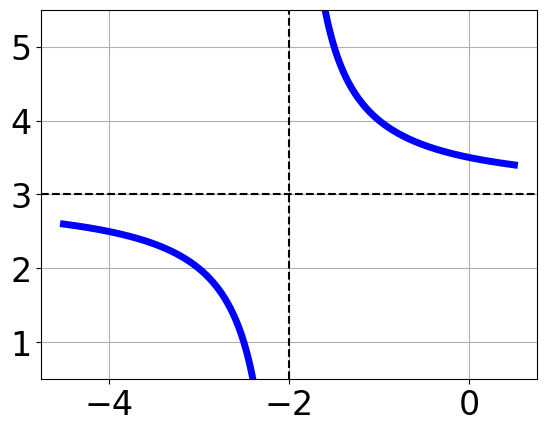
\includegraphics[width=0.3\textwidth]{../Figures/rationalGraphToEquationA.png} \end{center} 

The solution is $ f(x) = \frac{1}{x - 1} - 2 $ 

\begin{enumerate}[label=\Alph*.] 
\item $ f(x) = \frac{-1}{x + 1} - 2 $ 

 Corresponds to using the general form $f(x) = \frac{a}{x+h}+k$ and the opposite leading coefficient. 
\item $ f(x) = \frac{-1}{(x + 1)^2} - 2 $ 

 Corresponds to thinking the graph was a shifted version of $\frac{1}{x^2}$, using the general form $f(x) = \frac{a}{x+h}+k$, and the opposite leading coefficient. 
\item $ f(x) = \frac{1}{x - 1} - 2 $ 

 This is the correct option. 
\item $ f(x) = \frac{1}{(x - 1)^2} - 2 $ 

 Corresponds to thinking the graph was a shifted version of $\frac{1}{x^2}$. 
\item $ \text{None of the above} $ 

 This corresponds to believing the vertex of the graph was not correct. 
\end{enumerate} 
 
General Comments: Remember that the general form of a basic rational equation is $ f(x) = \frac{a}{(x-h)^n} + k$, where $a$ is the leading coefficient (and in this case, we assume is either $1$ or $-1$), $n$ is the degree (in this case, either $1$ or $2$), and $(h, k)$ is the intersection of the asymptotes.

-----------------------------------------------


\end{document}

